Le Tome I définit un système autonome : ses états, sa trace, son graphe et ses événements internes. Il rappelle également le paysage autonome utilisé ici : plusieurs attracteurs peuvent coexister et le bassin atteint dépend de la condition initiale.

Le Tome II ajoute un autre système ou un monde extérieur. La difficulté n'est pas seulement d'ajouter une entrée. Il faut préciser par quel canal cette entrée agit et distinguer trois situations :

\begin{enumerate}
\def\labelenumi{\arabic{enumi}.}
\tightlist
\item
  l'influence modifie temporairement la dynamique, mais le système revient au même attracteur autonome ;
\item
  le système produit une réponse qui compense partiellement l'influence sans changer de bassin ;
\item
  après la fin de l'interaction, le système atteint un attracteur autonome différent.
\end{enumerate}

Ces trois situations seront appelées \textbf{inertie},
\textbf{résistance} et \textbf{appropriation}.

Une deuxième difficulté apparaît lorsque l'interface possède sa propre dynamique. L'intensité reçue peut alors être filtrée, accumulée ou écrite seulement lors d'événements discrets. Deux expositions de même durée et de même intensité ne produisent plus nécessairement la même réponse. Leur cadence, la phase du système au moment de la réception et les modifications persistantes de l'interface deviennent des variables du problème.

Le Tome II procède en trois étapes :

\[
\text{influence continue}
\longrightarrow
\text{interface dynamique}
\longrightarrow
\text{mémoire de l'interface}.
\]

\part{De l’influence à l’appropriation}
\chapter{Axiomes minimaux de l'interface}\label{t2-axiomes-minimaux-de-linterface}

Les axiomes suivants ne définissent pas encore une interface unique. Ils
précisent les contraintes que les modèles étudiés doivent respecter.

\section{Projection de l'état {[}CHOIX{]}}\label{t2-projection-de-letat-choix}

Un système \(B\) ne reçoit pas directement la trace, le préconditionneur
ou le graphe interne d'un système \(A\). Le couplage passe par une
projection de l'état de \(A\).

Dans la dyade minimale, cette projection est simplement

\[
\pi(h_A)=\sigma(h_A),
\]

avec \(\sigma=\tanh\) appliquée composante par composante.

Ainsi, \(B\) n'a pas accès à \(\tau_A\). La mémoire de \(A\) reste
privée par son support. Elle peut néanmoins être partiellement
observable par ses effets sur \(h_A\), par exemple à travers une vitesse
de relaxation ou une amplitude persistante.

\section{Co-modification de l'interface {[}CHOIX{]}}\label{t2-co-modification-de-linterface-choix}

L'interface peut porter un état propre. Cet état est modifié par ce qui
la traverse et agit ensuite sur les interactions suivantes.

Deux réalisations seront étudiées :

\begin{itemize}
\tightlist
\item
  une perméabilité \(q\), qui module l'amplitude de l'écriture ;
\item
  une variable lente \(s\), qui modifie la taille des quanta écrits lors
  des événements.
\end{itemize}

La présence d'une variable d'interface n'implique pas qu'elle soit
indépendante du système. Elle est une composante supplémentaire de la
dynamique couplée.

\section{Intégration conditionnelle {[}CHOIX{]}}\label{t2-integration-conditionnelle-choix}

Une influence n'est pas nécessairement intégrée au moment où elle
atteint l'interface.

Dans le modèle R2 minimal, elle est d'abord accumulée dans une variable
\(\chi\), puis écrite dans la trace lors d'un Kairos. Cette première
version rend l'écriture événementielle, mais pas encore conditionnelle :
tout quantum présent au moment de l'événement est écrit.

La version directionnelle introduite plus loin ajoute un critère de
compatibilité. La quantité écrite dépend alors de l'accord entre la
mémoire lente de l'interface et l'influence présente.

\section{L'influence agit par la trace {[}CHOIX{]}}\label{t2-linfluence-agit-par-la-trace-choix}

L'autre système n'apparaît pas comme une force ajoutée directement à
l'équation de l'état rapide. Il écrit dans la trace du système receveur.
Cette trace modifie ensuite le rappel et la dissipation.

La chaîne causale est donc :

\[
\text{état extérieur}
\longrightarrow
\text{écriture dans la trace}
\longrightarrow
\text{modification du rappel}
\longrightarrow
\text{évolution de l'état}.
\]

Cette contrainte est importante. Elle permet de distinguer une influence
qui ouvre une possibilité dynamique d'une force qui déplacerait
directement le système.

\chapter{La dyade minimale}\label{t2-la-dyade-minimale}

\section{Deux systèmes réduits}\label{t2-deux-systemes-reduits}

On considère deux systèmes \(A\) et \(B\) sur la variété homogène du
Tome I. Chaque système possède un état \(h_X\), une vitesse \(v_X\) et
une trace \(\tau_X\), avec \(X\in\{A,B\}\).

La dynamique interne est

\[
\dot h_X=v_X,
\]

\[
\dot v_X
=
-\Gamma(\tau_X)v_X
-
M(\tau_X)h_X
+
\zeta\,\sigma(h_X).
\]

Pour une influence unidirectionnelle de \(A\) vers \(B\),

\[
\dot\tau_B
=
\alpha\,\sigma(h_B)
+
g\,\sigma(h_A)
-
\beta\tau_B.
\]

Le paramètre \(g\geq0\) mesure l'intensité du couplage. Le système \(A\)
est placé sur un attracteur actif et joue le rôle de source. Le système
\(B\) est initialement proche du repos.

\section{Réduction scalaire}\label{t2-reduction-scalaire}

L'analyse principale utilise la diagonale de dimension \(d=2\). On écrit

\[
h_B=(x,x),
\qquad
v_B=(v,v),
\qquad
\tau_B=(\theta,\theta).
\]

Le système source est fixé sur son puits positif et

\[
w=\tanh(x_A)=0{,}98006.
\]

La dynamique de \(B\) devient

\[
\dot x=v,
\]

\[
\dot v
=
-\Gamma(\sqrt2|\theta|)v
-
m(\sqrt2|\theta|)x
+
\zeta\tanh x,
\]

\[
\dot\theta
=
\alpha\tanh x
+
gw
-
\beta\theta.
\]

Ici, \(m(r)\) est la valeur propre du préconditionneur dans la direction
de la trace :

\[
m(r)
=
\frac{1+r^2}{1+(1+\lambda)r^2}.
\]

Elle décroît de \(1\) vers \((1+\lambda)^{-1}\).

Cette réduction est exacte tant que la trajectoire reste sur la
diagonale. Elle ne décrit pas les perturbations transverses ni les
dyades asymétriques.

\chapter{L'influence ne déplace pas directement le repos}\label{t2-linfluence-ne-deplace-pas-directement-le-repos}

Considérons la condition

\[
x(0)=0,
\qquad
v(0)=0.
\]

Même si \(g>0\), on a

\[
\dot v
=
-\Gamma(\sqrt2|\theta|)\,0
-
m(\sqrt2|\theta|)\,0
+
\zeta\tanh 0
=0.
\]

La trace peut augmenter sous l'effet du terme \(gw\), mais l'état reste
exactement nul.

\begin{quote}
\resultheading{Proposition}{prop:t2-repos-invariant}{ \texttt{{[}PROP{]}}} Pour toute trajectoire
admissible de la trace, l'ensemble \[
\{x=0,\ v=0\}
\] est invariant.
\end{quote}

L'influence modifie donc la stabilité du repos sans créer elle-même un
déplacement. Une perturbation initiale, même très petite, reste
nécessaire pour quitter l'ensemble invariant.

La linéarisation en \((x,v)=(0,0)\) est

\[
\frac{\mathrm d}{\mathrm dt}
\begin{pmatrix}
x\\ v
\end{pmatrix}
=
\begin{pmatrix}
0 & 1\\
\zeta-m(\sqrt2|\theta(t)|)
&
-\Gamma(\sqrt2|\theta(t)|)
\end{pmatrix}
\begin{pmatrix}
x\\ v
\end{pmatrix}.
\]

Pour une valeur momentanément fixée de la trace, le repos linéarisé perd sa stabilité lorsque

\[
m(\sqrt2|\theta|)<\zeta.
\]

On note \(\tau_{\mathrm{ign}}\) la norme de trace pour laquelle

\[
m(\tau_{\mathrm{ign}})=\zeta.
\]

Pour les paramètres de référence,

\[
\tau_{\mathrm{ign}}=0{,}3780.
\]

L'extérieur ne pousse donc pas \(B\) hors du repos. Il modifie le
coefficient de rappel jusqu'à rendre une perturbation existante
contractante ou croissante.

\chapter{Trois réponses à une influence continue}\label{t2-trois-reponses-a-une-influence-continue}

\section{Seuil local du repos}\label{t2-seuil-local-du-repos}

Si \(B\) reste exactement au repos, sa trace converge vers

\[
\theta_\infty=\frac{gw}{\beta}.
\]

Le seuil auquel le repos perd sa stabilité vérifie

\[
\sqrt2\,\theta_\infty=\tau_{\mathrm{ign}}.
\]

On obtient

\[
\boxed{
g_c
=
\frac{\beta\tau_{\mathrm{ign}}}{\sqrt2\,w}
=
0{,}03273
}.
\]

Ce seuil est local : il indique un changement de stabilité du repos. Il
ne détermine pas à lui seul l'attracteur atteint par une condition
initiale donnée.

\section{Inertie}\label{t2-inertie}

Pour

\[
g<g_c,
\]

la charge stationnaire reste sous le seuil d'instabilité. Une petite
perturbation décroît et le système revient au repos.

Dans ce régime, une exposition peut modifier la trace sans modifier
l'attracteur autonome atteint après découplage.

\section{Résistance}\label{t2-resistance}

Pour \(g\) légèrement supérieur à \(g_c\), le système ne se dirige pas
nécessairement vers le puits positif. Une branche d'équilibres apparaît
du côté négatif :

\[
x_{\mathrm{res}}(g)<0.
\]

L'état de \(B\) devient donc antiparallèle à l'influence reçue. Cette
réponse produit une contre-écriture

\[
\alpha\tanh(x_{\mathrm{res}})<0
\]

qui compense une partie de la charge externe \(gw\).

À l'équilibre,

\[
\beta\theta^\ast
=
\alpha\tanh(x^\ast)+gw
\]

et

\[
m(\sqrt2|\theta^\ast|)x^\ast
=
\zeta\tanh(x^\ast).
\]

Pour \(x^\ast\neq0\),

\[
m(\sqrt2|\theta^\ast|)
=
\zeta\frac{\tanh x^\ast}{x^\ast}
<\zeta.
\]

La branche ne maintient donc pas exactement \(m=\zeta\). Elle s'en
approche au voisinage de l'origine :

\[
m(\sqrt2|\theta^\ast|)
=
\zeta-\frac{\zeta}{3}(x^\ast)^2+o((x^\ast)^2).
\]

La résistance place le système près de la marge d'instabilité, avec un
écart quadratique en \(x^\ast\).

\section{Appropriation}\label{t2-appropriation}

Pour certaines intensités et certains protocoles, la trajectoire échappe
à la branche résistante, traverse la séparatrice autonome et atteint le
puits positif.

Après la fin du couplage, le système reste dans ce puits. L'état atteint
est un attracteur propre à \(B\), non une copie maintenue de l'état de
\(A\).

La différence entre résistance et appropriation ne porte donc pas
seulement sur l'amplitude observée pendant l'exposition. Elle porte sur
le bassin autonome atteint après le découplage.

\chapter{La branche résistante}\label{t2-la-branche-resistante}

\section{Naissance par bifurcation transcritique}\label{t2-naissance-par-bifurcation-transcritique}

Les équilibres sont les zéros du résidu

\[
F_g(x)
=
m(\sqrt2|\theta^\ast(x,g)|)x
-
\zeta\tanh x,
\]

avec

\[
\theta^\ast(x,g)
=
\frac{\alpha\tanh x+gw}{\beta}.
\]

L'origine est une racine pour tout \(g\). Au voisinage de
\((x,g)=(0,g_c)\),

\[
F_g(x)
=
x\left[
a_1(g-g_c)
+
a_2x
+
a_3x^2
+
\cdots
\right],
\]

avec

\[
a_1<0,
\qquad
a_2<0.
\]

Comme \(a_2\neq0\), l'origine et la branche non nulle se croisent dans
une bifurcation transcritique \citep{kuznetsov2004elements}.

\begin{quote}
\resultheading{Proposition}{prop:t2-branche-resistante}{ \texttt{{[}PROP-NUM{]}}} Une branche d'équilibres
résistants traverse l'origine en \(g=g_c\). Elle se situe du côté
\(x<0\) pour \(g>g_c\).
\end{quote}

\section{Développement local}\label{t2-developpement-local}

Le premier ordre est

\[
x_{\mathrm{res}}(g)
=
-\frac{w}{\alpha}(g-g_c)
+
O((g-g_c)^2).
\]

Le coefficient \(-w/\alpha\) vient de la compensation entre la charge
extérieure et la contre-écriture produite par \(B\).

Le développement au second ordre, pour les paramètres de référence, est

\[
\boxed{
x_{\mathrm{res}}(g)
=
-2{,}1774(g-g_c)
+
0{,}3216(g-g_c)^2
+
O((g-g_c)^3)
}.
\]

La faible valeur du coefficient quadratique résulte d'une
quasi-annulation entre trois contributions du développement. L'origine
générale de cette compensation n'est pas encore établie.

\section{Stabilité et rupture de type Hopf}\label{t2-stabilite-et-rupture-par-hopf}

La branche résistante est stable sur l'intervalle numérique

\[
g_c<g<g_H,
\qquad
g_H=0{,}1285.
\]

À \(g_H\), une paire de valeurs propres complexes traverse l'axe
imaginaire. La pulsation mesurée est

\[
\omega_H\simeq0{,}334,
\]

soit une période d'environ \(18{,}8\).

Ce franchissement possède la signature spectrale d'une bifurcation de Hopf. La transversalité est vérifiée numériquement ; le premier coefficient de Lyapunov n'étant pas encore calculé, la nature locale complète de la bifurcation n'est pas établie \citep{kuznetsov2004elements}.

La racine résistante ne disparaît pas à \(g_H\). Elle persiste au-delà, mais devient instable. Par exemple, à \(g=0{,}145\),

\[
x_{\mathrm{res}}=-0{,}2453
\]

et la partie réelle maximale du spectre vaut \(0{,}0036>0\).

\begin{quote}
\resultheading{Proposition}{prop:t2-rupture-hopf}{ \texttt{{[}PROP-NUM{]}}} La branche résistante existe au-delà de \(g_H\), mais elle perd sa stabilité à \(g_H\). Dans les simulations de référence, la trajectoire quitte alors son voisinage et atteint le puits positif.
\end{quote}

La nature sous-critique ou surcritique de la bifurcation n'est pas encore déterminée.

\chapter{Trois seuils qui ne décrivent pas le même phénomène}\label{t2-trois-seuils-phenomenes-distincts}
\chaptermark{Trois seuils distincts}

Les calculs précédents font apparaître trois valeurs distinctes.

\section{\texorpdfstring{\(g_c\)}{gc} : seuil de stabilité locale}\label{t2-g_c-seuil-de-stabilite-locale}

\[
g_c=0{,}0327
\]

est le seuil transcritique. Le repos perd sa stabilité locale et la
branche résistante apparaît.

\section{\texorpdfstring{\(g_{\mathrm{ign}}\)}{g ign} : seuil de capture pour un protocole}\label{t2-g_mathrmign-seuil-de-capture-pour-un-protocole}

Pour la condition initiale standard

\[
x_0=10^{-3},
\qquad
v_0=0,
\qquad
\theta_0=0,
\]

et une mise sous contact brutale, le changement d'issue se produit vers

\[
g_{\mathrm{ign}}\simeq0{,}0556.
\]

Ce seuil n'est pas une bifurcation. À \(g_{\mathrm{ign}}+\varepsilon\), une condition initiale placée sur la branche résistante y reste, alors que la condition initiale standard s'en échappe.

Il faut donc écrire

\[
g_{\mathrm{ign}}
=
g_{\mathrm{ign}}(x_0,\theta_0,v_0;\mathcal P),
\]

où \(\mathcal P\) désigne le protocole de mise sous contact.

Cette dépendance est visible à \(g=0{,}10\) :

\begin{itemize}
\tightlist
\item
  une exposition brutale conduit à l'appropriation ;
\item
  une rampe courte conduit également à l'appropriation ;
\item
  une rampe lente de durée \(400\) permet à la trajectoire de suivre la
  branche résistante.
\end{itemize}

La montée progressive protège ici le système parce qu'elle laisse le temps au transitoire de se rapprocher de la branche stable.

\section{\texorpdfstring{\(g_H\)}{gH} : seuil de stabilité de la branche}\label{t2-g_h-seuil-de-stabilite-de-la-branche}

\[
g_H=0{,}1285
\]

est le seuil auquel la branche résistante perd sa stabilité. Il ne
dépend pas de la condition initiale de la même manière que
\(g_{\mathrm{ign}}\).

La hiérarchie est donc

\[
\boxed{
g_c
<
g_{\mathrm{ign}}(x_0,\theta_0,v_0;\mathcal P)
<
g_H
}
\]

pour le protocole de référence.

\begin{figure}[!htbp]
\centering
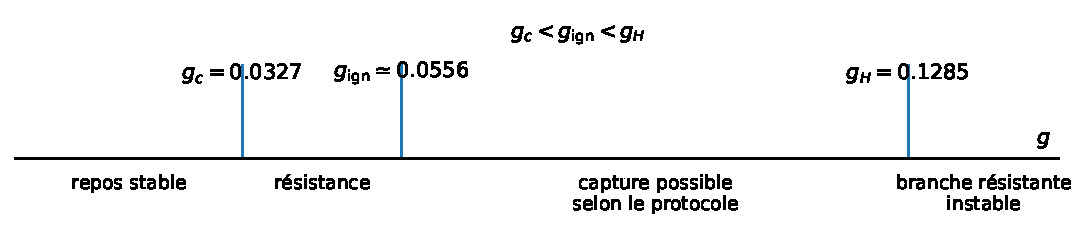
\includegraphics[width=0.96\textwidth]{fig/scientifiques/figure_trois_seuils.pdf}
\caption{Les trois seuils du protocole de référence sur un même axe. Le seuil transcritique $g_c$ et le seuil de perte de stabilité $g_H$ caractérisent la dynamique locale des branches, tandis que $g_{\mathrm{ign}}$ est un seuil de capture dépendant de la condition initiale et du protocole $\mathcal P$. La figure visualise donc une hiérarchie de mécanismes, et non trois bifurcations de même nature.}
\label{fig:t2-trois-seuils}
\end{figure}

\chapter{Définition et loi d'appropriation}\label{t2-definition-et-loi-dappropriation}

\section{Définition par les bassins {[}DEF{]}}
\label{t2-definition-par-les-bassins-def}

Soit \(z_0\) l'état de \(B\) avant l'interaction. On applique le
couplage d'intensité \(g\) pendant une durée \(T\), selon un protocole
\(\mathcal P\), puis on supprime ce couplage.

On note

\[
y_T
=
\Phi_{g,\mathcal P}^{T}(z_0)
\]

l'état obtenu au moment du découplage, et \(\omega_0(z)\) l'ensemble
limite de la dynamique autonome issue de \(z\).

\begin{quote}
\resultheading{Définition}{def:t2-appropriation}{} L'interaction \((g,T,\mathcal P)\) est appropriée
depuis \(z_0\) si

\[
\omega_0(y_T)=\mathcal A,
\qquad
\omega_0(z_0)=\mathcal A_0,
\qquad
\mathcal A\neq\mathcal A_0,
\]

où \(\mathcal A_0\) et \(\mathcal A\) sont des attracteurs autonomes de
\(B\).
\end{quote}

Cette définition exclut trois situations :

\begin{itemize}
\tightlist
\item
  une réponse temporaire qui disparaît après découplage ;
\item
  une copie maintenue uniquement par la présence de \(A\) ;
\item
  une transmission directe de la mémoire interne de \(A\).
\end{itemize}

\section{Durée minimale d'exposition}
\label{t2-duree-minimale-dexposition}

Pour une intensité \(g\), une condition initiale \(z_0\) et un protocole
\(\mathcal P\), on définit

\[
T^\ast(g;z_0,\mathcal P)
=
\inf
\left\{
T>0 :
(g,T,\mathcal P)
\text{ est appropriée depuis }z_0
\right\}.
\]

Lorsque cet ensemble est vide,

\[
T^\ast=+\infty.
\]

La notation abrégée

\[
T^\ast(g)
\]

suppose donc que la condition initiale et le protocole sont fixés.

\section{Linéarisation le long de la trace}\label{t2-linearisation-le-long-de-la-trace}

Près du repos, on linéarise la dynamique de \((x,v)\) le long de la
trajectoire temporelle de la trace :

\[
\dot z=A(t)z,
\qquad
z=
\begin{pmatrix}
x\\ v
\end{pmatrix},
\]

\[
A(t)
=
\begin{pmatrix}
0 & 1\\
\zeta-m(\sqrt2|\theta(t)|)
&
-\Gamma(\sqrt2|\theta(t)|)
\end{pmatrix}.
\]

Pendant l'exposition, \(\theta(t)\) augmente sous l'effet du terme
\(gw\). Après le découplage, elle décroît.

Lorsque

\[
m(\sqrt2|\theta(t)|)<\zeta,
\]

le coefficient linéaire de \(x\) devient positif. La petite perturbation
initiale peut alors croître.

Le calcul prédit une appropriation lorsque la trajectoire linéarisée
atteint le voisinage de l'équilibre-selle autonome positif

\[
x_u=0{,}0717
\]

avant que la décroissance de la trace ne referme la fenêtre
d'instabilité.

Ce prédicteur n'utilise pas de paramètre ajusté aux simulations.

\begin{longtable}[]{@{}rrr@{}}
\toprule\noalign{}
\(g\) & \(T^\ast\) prédit & \(T^\ast\) mesuré \\
\midrule\noalign{}
\endhead
\bottomrule\noalign{}
\endlastfoot
0,05 & aucune durée dans le régime étudié & aucune \\
0,08 & 31,6 & 31,7 \\
0,10 & 24,8 & 24,8 \\
0,15 & 17,8 & 17,9 \\
0,20 & 14,9 & 15,0 \\
0,30 & 12,2 & 12,3 \\
\end{longtable}

\begin{figure}[H]
\centering
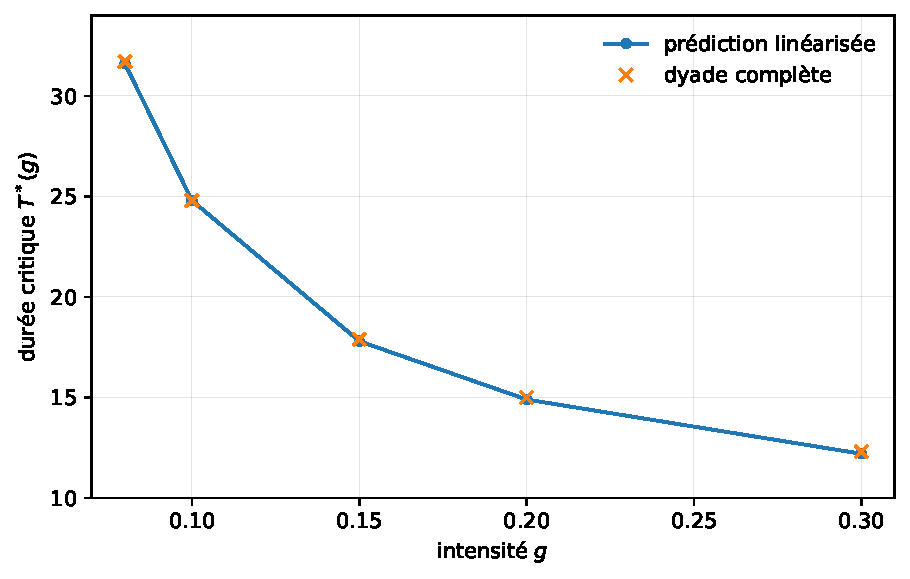
\includegraphics[width=0.90\textwidth]{fig/scientifiques/figure_duree_appropriation.pdf}
\caption{Durée critique d'appropriation pour le protocole de référence. Les points issus de la dyade complète restent au voisinage de la prédiction linéarisée, sans ajustement sur les simulations. Les valeurs numériques et le protocole de mesure sont détaillés à l'Annexe~\ref{annexe-branche-resistante-appropriation}.}
\label{fig:t2-duree-appropriation}
\end{figure}

L'écart reste inférieur à \(0{,}5\,\%\) pour les valeurs testées.

Dans la zone de résistance, prolonger l'exposition ne conduit pas à l'appropriation selon le protocole de référence. Pendant le contact, la trajectoire est capturée par la branche résistante ; après le découplage, elle revient au repos autonome.

L'analyse des trois seuils, la définition de l'appropriation par les bassins et la construction du prédicteur \(T^\ast\) sont détaillées à l'Annexe~\ref{annexe-branche-resistante-appropriation}.

\chapter{Couplage mutuel : alliance et compétition}\label{t2-couplage-mutuel-alliance-et-competition}

L'influence unidirectionnelle suffit pour définir la résistance et l'appropriation. Un couplage bidirectionnel fait apparaître deux réductions supplémentaires.

Ces réductions sont exactes sous trois conditions :

\begin{itemize}
\tightlist
\item
  les deux systèmes ont les mêmes paramètres ;
\item
  les couplages sont symétriques ;
\item
  la trajectoire reste dans le sous-espace aligné ou antipodal considéré.
\end{itemize}

\section{États alignés}\label{t2-etats-alignes}

Si

\[
h_B=h_A,
\]

alors les écritures interne et extérieure s'ajoutent :

\[
\dot\tau
=
(\alpha+g)\sigma(h)-\beta\tau.
\]

Le couplage se ramène à la transformation

\[
\alpha_{\mathrm{eff}}=\alpha+g.
\]

Pour \(g=0{,}2\), la frontière d'existence des puits actifs passe de

\[
\zeta_{\min}=0{,}3986
\]

à

\[
\zeta_{\min}=0{,}3772.
\]

Le puits commun prédit vaut \(3{,}3116\), contre \(3{,}312\) mesuré.

Le couplage aligné stabilise donc les états actifs communs dans ce
sous-espace.

\section{États antipodaux}\label{t2-etats-antipodaux}

Si

\[
h_B=-h_A,
\]

alors

\[
\sigma(h_B)=-\sigma(h_A)
\]

et

\[
\dot\tau
=
(\alpha-g)\sigma(h)-\beta\tau.
\]

Le couplage se ramène à

\[
\alpha_{\mathrm{eff}}=\alpha-g.
\]

La branche antipodale disparaît lorsque

\[
\zeta_{\min}\!\left(\frac{\alpha-g}{\beta}\right)=\zeta.
\]

Pour les paramètres de référence,

\[
g_{\mathrm{comp}}=0{,}3757.
\]

Sous ce seuil, les deux états opposés coexistent avec des puits moins profonds. Au-dessus, la configuration antipodale n'est plus disponible. Une symétrie exacte peut conduire les deux systèmes au repos. Dans les simulations, une petite asymétrie conduit généralement à leur capture dans le même puits.

Ces résultats ne couvrent pas les couplages asymétriques ni les systèmes ayant des paramètres différents.


\part{Quand l’interface devient dynamique}
\chapter{R1 : perméabilité dynamique}\label{t2-r1-permeabilite-dynamique}

Le modèle continu R0 écrit immédiatement l'influence dans la trace. R1
ajoute une variable \(q\in[0,1]\) qui représente la part effectivement
transmise.

\section{Équation de perméabilité}\label{t2-equation-de-permeabilite}

On pose

\[
\dot q
=
\rho(1-q)
-
\eta qgw.
\]

Le premier terme rouvre progressivement l'interface. Le second réduit sa
perméabilité lorsque le trafic est soutenu.

L'écriture dans la trace devient

\[
qg\,\sigma(h_A).
\]

À couplage constant,

\[
q_\infty
=
\frac{\rho}{\rho+\eta gw}
\]

et l'intensité transmise à long terme est

\[
\boxed{
g_{\mathrm{eff}}(g)
=
q_\infty g
=
\frac{\rho g}{\rho+\eta gw}
}.
\]

Elle satisfait

\[
\lim_{g\to\infty}g_{\mathrm{eff}}(g)
=
\frac{\rho}{\eta w}.
\]

\section{Transport des seuils}\label{t2-transport-des-seuils}

Soit \(g_\star^0\) un seuil du modèle continu R0. Le seuil
quasi-statique de R1 vérifie

\[
g_{\mathrm{eff}}(g_\star^{R1})=g_\star^0.
\]

On obtient

\[
\boxed{
g_\star^{R1}
=
\frac{\rho g_\star^0}
{\rho-\eta w g_\star^0}
}
\]

si

\[
\rho>\eta w g_\star^0.
\]

Dans le cas contraire, le seuil est inaccessible : la saturation de
\(g_{\mathrm{eff}}\) reste sous \(g_\star^0\).

Pour

\[
\rho=0{,}05,
\qquad
\eta=1,
\]

la formule donne

\[
g_c^{R1}=0{,}0913.
\]

Le seuil observé dynamiquement est \(0{,}0863\). La différence vient de
la condition initiale \(q(0)=1\) : le système bénéficie d'une fenêtre de
forte ouverture avant que l'interface ne se ferme.

\section{Protection de la résistance}\label{t2-protection-de-la-resistance}

Avec les mêmes paramètres,

\[
\frac{\rho}{\eta w}=0{,}0510<g_H^0.
\]

Le couplage effectif soutenu ne peut donc pas atteindre le seuil de Hopf
du modèle continu. R1 rend cette rupture inaccessible par une simple
augmentation de \(g\).

Cette protection est structurelle pour la loi de perméabilité choisie.
Elle ne prouve pas que toute interface dynamique protège la branche
résistante.

\section{Effet sur la durée d'exposition}\label{t2-effet-sur-la-duree-dexposition}

R1 allonge la durée nécessaire à l'appropriation :

\begin{longtable}[]{@{}rrr@{}}
\toprule\noalign{}
\(g\) & \(T^\ast\) sous R0 & \(T^\ast\) sous R1 \\
\midrule\noalign{}
\endhead
\bottomrule\noalign{}
\endlastfoot
0,10 & 24,8 & 88,9 \\
0,20 & 15,0 & 32,1 \\
0,30 & 12,3 & 26,2 \\
\end{longtable}

La loi R1 minimale ne produit pas d'hystérésis propre en régime stationnaire : pour chaque valeur fixée de \(g\), la dynamique de \(q\) possède un unique équilibre \(q_\infty(g)\), globalement stable.

Une hystérésis demanderait une loi supplémentaire, par exemple des seuils distincts ou plusieurs branches d'équilibre.

\chapter{R2 : écriture aux Kairos}\label{t2-r2-ecriture-aux-kairos}

R2 ne réduit pas directement l'amplitude. Il modifie le moment où
l'influence est écrite dans la trace.

\section{Accumulation à l'interface}\label{t2-accumulation-a-linterface}

L'influence s'accumule dans une variable \(\chi\) :

\[
\dot\chi
=
g\sigma(h_A)
-
\lambda_\chi\chi.
\]

Elle contribue à la pression événementielle :

\[
\dot p
=
\cdots
+
\kappa_\chi\|\chi\|.
\]

Au Kairos,

\[
\tau^+
=
\tau^-
+
\kappa_Q\chi^-,
\]

\[
\chi^+
=
(1-r_\chi)\chi^-,
\]

\[
p^+
=
r_Pp^-.
\]

Les paramètres de référence sont

\[
\lambda_\chi=0{,}2,
\qquad
\kappa_Q=0{,}6,
\qquad
r_\chi=0{,}8,
\qquad
\kappa_\chi=2{,}5.
\]

Cette version réalise une \textbf{écriture événementielle}. Elle ne
réalise pas encore une validation conditionnelle, car le quantum est
écrit quelle que soit son orientation.

\section{Validation et appropriation sont distinctes}\label{t2-validation-et-appropriation-sont-distinctes}

À \(g=0{,}10\), le protocole produit \(271\) Kairos et une trace
maximale supérieure au seuil d'instabilité, sans changement de bassin
autonome.

Le nombre d'événements ne mesure donc pas l'appropriation. Les
événements transportent la charge, mais l'issue dépend encore de la
trajectoire dans l'espace des états et de sa position par rapport aux
séparatrices.

\chapter{Application de retour du cycle événementiel}\label{t2-application-de-retour-du-cycle-evenementiel}

\section{Cycle au repos}\label{t2-cycle-au-repos}

Au repos exact,

\[
x=0,
\qquad
v=0,
\]

la dynamique de \((\chi,p)\) est autonome. Pour les paramètres étudiés et \(g>g_K\), la résolution numérique met en évidence un cycle attractif d'événements de période \(\Delta(g).\)

Entre deux Kairos, \(\chi\) suit une loi exponentielle. La condition
\(p=\Theta\) qui définit le prochain événement conduit à une équation
transcendante pour \(\Delta\).

La carte est donc explicite une fois \(\Delta\) connu, mais \(\Delta\)
doit être calculé numériquement.

\section{Carte de la trace}\label{t2-carte-de-la-trace}

Si \(\chi_\ast^-\) désigne la charge immédiatement avant un événement sur le cycle, la composante scalaire de la trace vérifie

\[
\theta_{n+1}^+
=
e^{-\beta\Delta}\theta_n^+
+
\kappa_Q\chi_\ast^-.
\]

Son point fixe est

\[
\boxed{
\theta_\infty^+
=
\frac{\kappa_Q\chi_\ast^-}
{1-e^{-\beta\Delta}}
}.
\]

La moyenne temporelle de la trace sur un cycle vaut

\[
\boxed{
\bar\theta
=
\frac{\kappa_Q\chi_\ast^-}
{\beta\Delta}
}.
\]

Cette relation donne une charge continue équivalente :

\[
\text{charge moyenne}
=
\frac{\text{quantum par événement}}
{\text{période des événements}\times\text{taux d'oubli}}.
\]

Les valeurs prédites et mesurées concordent à environ \(10^{-4}\) sur
les quatre intensités testées.

\section{Stabilité du repos}\label{t2-stabilite-du-repos}

Dans la réduction R2 considérée, la dynamique linéaire de \((x,v)\) sur le cycle est périodique. Sa stabilité est déterminée par la matrice de monodromie, c'est-à-dire par l'évolution linéaire sur une période complète.

Le cycle réduit perd sa stabilité lorsque son multiplicateur dominant traverse le cercle unité \citep{goebel2012hybrid, lakshmikantham1989impulsive}.

Le calcul donne

\[
g_F=0{,}0763.
\]

Le critère quasi-statique

\[
\bar\theta=\theta_{\mathrm{ign}}
\]

donne

\[
g_F^{qs}=0{,}0760.
\]

L'écart est de \(0{,}4\,\%\). Le cycle événementiel est suffisamment
rapide devant l'évolution de la trace pour que le modèle continu moyenné
reste une bonne approximation locale.

\chapter{Les seuils de R2}\label{t2-les-seuils-de-r2}

Quatre phénomènes doivent être séparés.

\begin{longtable}[]{@{}
  >{\raggedright\arraybackslash}p{(\columnwidth - 4\tabcolsep) * \real{0.3000}}
  >{\raggedleft\arraybackslash}p{(\columnwidth - 4\tabcolsep) * \real{0.4000}}
  >{\raggedright\arraybackslash}p{(\columnwidth - 4\tabcolsep) * \real{0.3000}}@{}}
\toprule\noalign{}
\begin{minipage}[b]{\linewidth}\raggedright
Objet
\end{minipage} & \begin{minipage}[b]{\linewidth}\raggedleft
Valeur de référence
\end{minipage} & \begin{minipage}[b]{\linewidth}\raggedright
Signification
\end{minipage} \\
\midrule\noalign{}
\endhead
\bottomrule\noalign{}
\endlastfoot
\(g_K\) & 0,03608 & apparition d'une activité événementielle soutenue \\
\(g_F\) & 0,0763 & perte de stabilité locale du cycle R2 réduit \\
\(g_{\mathrm{app}}^{R2}(x_0;\mathcal P)\) & 0,1632 & appropriation pour
la perturbation initiale et le protocole de référence \\
\(g_H^{R2}\) & \(>0{,}30\) & aucune perte de stabilité de la résistance pulsée observée jusqu'à cette borne \\ & non observée jusqu'à 0,30 & seuil éventuel non identifié \\
\end{longtable}

Le seuil \(g_K\) possède la formule

\[
g_K
=
\frac{\Theta\kappa_3\lambda_\chi}
{\kappa_\chi\sqrt2\,w}.
\]

La valeur

\[
g_{\mathrm{app}}^{R2}=0{,}1632
\]

n'est pas un analogue de \(g_c\). Elle dépend d'une condition initiale,
d'un protocole et de la cadence endogène des événements.

Enfin, les simulations ne montrent aucune perte de stabilité de la
résistance pulsée jusqu'à \(g=0{,}30\). On écrit donc

\[
g_H^{R2}>0{,}30
\]

au sens d'une borne numérique. Cette écriture ne suppose ni qu'un seuil existe au-delà, ni qu'il s'agisse nécessairement d'une bifurcation de Hopf.

Les calculs de R1 et R2, l'application de retour et le statut distinct des seuils \(g_K\), \(g_F\), \(g_{\mathrm{app}}^{R2}\) et \(g_H^{R2}\) sont détaillés à l'Annexe~\ref{annexe-interfaces-r1-r2}.

\chapter{Deux expositions : la phase de réception}\label{t2-deux-expositions-la-phase-de-reception}

\section{Protocole}\label{t2-protocole}

On applique deux expositions sous-critiques de même intensité et de même durée. Elles sont séparées par un délai \(D\).

Pour

\[
g=0{,}18,
\qquad
T_{\mathrm{sub}}=41{,}9,
\]

le balayage de \(D\) fait apparaître des bandes d'appropriation séparées
par des zones d'échec.

La période des bandes est voisine de

\[
14,
\]

à comparer à la période de la spirale libre autour du repos,

\[
\frac{2\pi}{\omega}=14{,}63,
\]

avec

\[
\omega^2=(1-\zeta)-\frac{\gamma_0^2}{4}.
\]

\section{Trois régimes}\label{t2-trois-regimes}

\subsection{Mémoire de charge}\label{t2-memoire-de-charge}

Pour

\[
D\lesssim10,
\]

la trace, la charge d'interface et la pression n'ont pas encore disparu.
Leur amplitude domine l'effet de phase.

\subsection{Mémoire de phase}\label{t2-memoire-de-phase}

Pour

\[
10\lesssim D\lesssim48,
\]

la charge résiduelle est faible, mais l'état conserve une phase dans sa
relaxation oscillante.

La seconde exposition ne rend le repos instable qu'après un temps de
charge

\[
t_c=4{,}74,
\]

mesuré indépendamment sur l'application de retour. La quantité
pertinente est donc l'état libre extrapolé au temps

\[
D+t_c.
\]

Le prédicteur est

\[
\boxed{
x_{\mathrm{lib}}(D+t_c)>0
}.
\]

Il classe correctement \(18\) cellules sur \(20\) dans le régime de
phase, sans ajustement effectué sur le scan des délais.

Les deux erreurs se trouvent aux bords des bandes.

\subsection{Extinction de l'effet}\label{t2-extinction-de-leffet}

Pour

\[
D\gtrsim50,
\]

l'amplitude résiduelle devient trop faible. Le signe seul ne suffit
plus. La capture dépend alors de l'amplitude et de la structure fine des
bassins.

\section{Pourquoi la période vaut \texorpdfstring{\(2\pi/\omega\)}{2 pi / omega}}\label{t2-pourquoi-la-periode-vaut-2piomega}

Dans une instabilité parfaitement symétrique, les deux signes de \(x\)
pourraient conduire vers deux puits opposés. On attendrait alors une
répétition tous les \(\pi/\omega\).

Ce n'est pas ce qui se produit ici.

Dans le protocole étudié :

\begin{itemize}
\tightlist
\item
  les trajectoires qui s'approprient atteignent le puits positif, autour
  de \(+2{,}30\) ;
\item
  les trajectoires arrivant du côté négatif sont capturées par la
  résistance pulsée et reviennent vers le repos.
\end{itemize}

Les deux demi-périodes ne sont donc pas équivalentes. La branche
résistante supprime une alternance sur deux, ce qui explique la période
complète

\[
2\pi/\omega.
\]

Près de l'extinction, une forme plus générale redevient nécessaire :

\[
A(D)\cos(\omega D+\varphi_0)
>
A_{\mathrm{crit}}.
\]

Dans le régime de phase, \(A_{\mathrm{crit}}\) est proche de zéro et le critère se réduit au signe. Près de \(D\simeq50\), l'amplitude redevient déterminante.

\chapter{La dose totale ne détermine pas l'issue}\label{t2-la-dose-totale-ne-determine-pas-lissue}

On définit la charge nette écrite pendant une exposition par

\[
Q_{\mathrm{net}}
=
\sum_n
\kappa_Q\chi_n^-.
\]

Deux délais donnent :

\[
Q_{\mathrm{net}}(D=14)=8{,}255,
\]

avec appropriation, et

\[
Q_{\mathrm{net}}(D=26)=8{,}322,
\]

sans appropriation.

La deuxième trajectoire reçoit une charge légèrement plus grande, mais revient au repos par la branche résistante.

\begin{quote}
\textbf{Résultat \texttt{{[}NUM{]}}.} Dans ce protocole, la quantité
totale livrée ne suffit pas à expliquer l'issue. La phase à laquelle
cette charge rencontre la dynamique interne est déterminante.
\end{quote}

Ce résultat ne signifie pas que la dose est sans effet. Il montre
qu'elle n'est pas une statistique suffisante du protocole.

\part{Ce qui reste d’une interaction}

\chapter{Amorçage par une variable lente de l'interface}\label{t2-amorcage-par-une-variable-lente-de-linterface}

R2 minimal ne conserve rien lorsque \(\tau\), \(\chi\), \(p\), \(x\) et \(v\) sont revenus à leur état de base. Pour qu'une exposition non appropriée modifie une interaction ultérieure, une variable doit persister après cet oubli.

\section{Mémoire scalaire}\label{t2-memoire-scalaire}

On introduit

\[
\dot s
=
\varepsilon_s(\chi-s),
\qquad
\varepsilon_s=0{,}005.
\]

La taille des quanta devient

\[
\kappa_Q(s)
=
\kappa_Q(1+c_ss),
\qquad
c_s=8.
\]

Après une première exposition sous-critique et un délai de \(300\), les variables transitoires sont revenues à des valeurs négligeables, mais

\[
s=0{,}0095.
\]

Le gain initial des quanta est alors supérieur de \(7{,}6\,\%\) à sa
valeur de base.

\section{Effet sur une seconde exposition}\label{t2-effet-sur-une-seconde-exposition}

Pour les durées

\[
T_2=40,\ldots,155,
\]

on observe :

\begin{longtable}[]{@{}
  >{\raggedright\arraybackslash}p{(\columnwidth - 4\tabcolsep) * \real{0.2727}}
  >{\raggedleft\arraybackslash}p{(\columnwidth - 4\tabcolsep) * \real{0.3636}}
  >{\raggedleft\arraybackslash}p{(\columnwidth - 4\tabcolsep) * \real{0.3636}}@{}}
\toprule\noalign{}
\begin{minipage}[b]{\linewidth}\raggedright
État initial de l'interface
\end{minipage} & \begin{minipage}[b]{\linewidth}\raggedleft
Cellules appropriées
\end{minipage} & \begin{minipage}[b]{\linewidth}\raggedleft
Première durée appropriante
\end{minipage} \\
\midrule\noalign{}
\endhead
\bottomrule\noalign{}
\endlastfoot
sans amorçage & 17/24 & environ 75 \\
amorçage scalaire complet & 24/24 & au plus 40 \\
\end{longtable}

La première exposition ne modifie pas immédiatement le bassin autonome,
mais elle réduit durablement la durée nécessaire à une appropriation
ultérieure.

\begin{quote}
\resultheading{Définition}{def:t2-amorcage-interface}{} Une exposition produit un \textbf{amorçage d'interface} si, après extinction des variables transitoires et sans changement immédiat de bassin autonome, elle modifie la réponse à une exposition ultérieure.
\end{quote}

\section{Tête d'avance et boucle dynamique}\label{t2-tete-davance-et-boucle-dynamique}

Un contrôle remplace la boucle dynamique par un gain constant égal au
gain initial produit par \(s\).

Les résultats sont :

\begin{longtable}[]{@{}lrr@{}}
\toprule\noalign{}
Modèle & Cellules appropriées & Première durée appropriante \\
\midrule\noalign{}
\endhead
\bottomrule\noalign{}
\endlastfoot
sans amorçage & 17 & 75 \\
gain constant \(+7{,}6\,\%\) & 23 & 45 \\
boucle complète & 24 & 40 \\
\end{longtable}

L'essentiel de l'amorçage vient donc de la tête d'avance présente au
début de la seconde exposition. La rétroaction, dans laquelle des quanta
plus grands alimentent ensuite \(s\), ajoute un effet secondaire.

La formulation correcte est :

\[
\text{amorçage}
=
\text{gain initial persistant}
+
\text{amplification dynamique secondaire}.
\]

\section{Temps fini et contact soutenu}\label{t2-temps-fini-et-contact-soutenu}

Le résidu de \(s\) modifie fortement la durée critique d'une rencontre
finie. Il modifie très peu le seuil d'appropriation sous contact soutenu
:

\[
\Delta g_{\mathrm{app}}\simeq-0{,}0014.
\]

Sur un temps suffisamment long, \(s\) se recharge dans les deux
conditions. La mémoire de l'interface change donc surtout ce qui est
accessible pendant la durée d'une interaction, non l'ensemble des
comportements possibles sous contact permanent.

\chapter{Limite de la mémoire scalaire}\label{t2-limite-de-la-memoire-scalaire}

La variable \(s\) précédente dépend de l'intensité de \(\chi\), pas de
sa direction. Elle mémorise qu'une exposition a eu lieu, sans distinguer
ce qui a été reçu.

Le contrôle directionnel confirme cette limite.

Après une amorce et un oubli, on applique une seconde exposition :

\begin{itemize}
\tightlist
\item
  dans la même direction ;
\item
  dans une direction orthogonale ;
\item
  dans la direction opposée.
\end{itemize}

La perturbation initiale de l'état est rétablie au début de la seconde exposition afin que sa décroissance pendant le délai ne masque pas l'effet de l'interface. Cette remise à la graine fait partie du protocole de contrôle.

Pour la mémoire scalaire :

\begin{longtable}[]{@{}lr@{}}
\toprule\noalign{}
Seconde exposition & Cellules appropriées \\
\midrule\noalign{}
\endhead
\bottomrule\noalign{}
\endlastfoot
même direction & 5/12 \\
orthogonale & 5/12 \\
opposée & 5/12 \\
base sans amorce & 2/12 \\
\end{longtable}

L'amorçage est global. Il facilite de la même manière les trois
directions.

\chapter{Mémoire directionnelle et compatibilité}\label{t2-memoire-directionnelle-et-compatibilite}

\section{Variable vectorielle}\label{t2-variable-vectorielle}

On remplace \(s\) par une variable vectorielle :

\[
\dot{\mathbf s}
=
\varepsilon_s(\boldsymbol\chi-\mathbf s).
\]

Elle conserve une direction moyenne des expositions récentes.

Au Kairos, la trace reçoit

\[
\boxed{
\tau^+
=
\tau^-
+
\max\!\left(
1+c_s\langle\mathbf s,\widehat{\boldsymbol\chi}\rangle,
0
\right)
\kappa_Q\boldsymbol\chi^-
}
\]

avec

\[
\widehat{\boldsymbol\chi}
=
\frac{\boldsymbol\chi}
{\|\boldsymbol\chi\|}
\]

lorsque \(\boldsymbol\chi\neq0\).

Le facteur de compatibilité dépend du produit scalaire entre la mémoire
lente de l'interface et l'exposition présente.

\section{Trois cas}\label{t2-trois-cas}

Si l'exposition présente est alignée avec \(\mathbf s\),

\[
\langle\mathbf s,\widehat{\boldsymbol\chi}\rangle>0,
\]

et le quantum est augmenté.

Si elle est orthogonale,

\[
\langle\mathbf s,\widehat{\boldsymbol\chi}\rangle=0,
\]

et le quantum conserve sa taille de base.

Si elle est opposée,

\[
\langle\mathbf s,\widehat{\boldsymbol\chi}\rangle<0,
\]

et le quantum est réduit.

La borne inférieure à zéro empêche une anti-écriture dans laquelle un
quantum inversé effacerait artificiellement la trace.

\section{Résultats}\label{t2-resultats}

\begin{longtable}[]{@{}
  >{\raggedright\arraybackslash}p{(\columnwidth - 8\tabcolsep) * \real{0.1579}}
  >{\raggedleft\arraybackslash}p{(\columnwidth - 8\tabcolsep) * \real{0.2105}}
  >{\raggedleft\arraybackslash}p{(\columnwidth - 8\tabcolsep) * \real{0.2105}}
  >{\raggedleft\arraybackslash}p{(\columnwidth - 8\tabcolsep) * \real{0.2105}}
  >{\raggedleft\arraybackslash}p{(\columnwidth - 8\tabcolsep) * \real{0.2105}}@{}}
\toprule\noalign{}
\begin{minipage}[b]{\linewidth}\raggedright
Mémoire de l'interface
\end{minipage} & \begin{minipage}[b]{\linewidth}\raggedleft
Même direction
\end{minipage} & \begin{minipage}[b]{\linewidth}\raggedleft
Orthogonale
\end{minipage} & \begin{minipage}[b]{\linewidth}\raggedleft
Opposée
\end{minipage} & \begin{minipage}[b]{\linewidth}\raggedleft
Base
\end{minipage} \\
\midrule\noalign{}
\endhead
\bottomrule\noalign{}
\endlastfoot
scalaire & 5/12 & 5/12 & 5/12 & 2/12 \\
vectorielle & 5/12 & 2/12 & 1/12 & 2/12 \\
\end{longtable}

La mémoire vectorielle produit donc :

\begin{itemize}
\tightlist
\item
  une facilitation pour une exposition de même direction ;
\item
  une neutralité mesurée pour une exposition orthogonale ;
\item
  une inhibition pour une exposition opposée.
\end{itemize}

Ces trois effets proviennent d'une seule règle. Ils ne sont pas
implémentés par trois mécanismes séparés.

Nous parlerons ici d'\textbf{inhibition directionnelle} plutôt que
d'habituation au sens strict. Une habituation demanderait de montrer
qu'une répétition du même signal réduit progressivement la réponse, ce
que ce protocole ne montre pas.

\section{Statut de l'intégration conditionnelle}\label{t2-statut-de-lintegration-conditionnelle}

R2 minimal écrivait tout quantum présent au Kairos. La règle vectorielle
introduit pour la première fois une condition calculée à partir de
l'histoire de l'interface.

Elle ne décide pas seulement si une écriture a lieu. Elle module le
canal futur selon la relation entre ce qui a été reçu et ce qui arrive
maintenant.

\begin{quote}
\textbf{Résultat \texttt{{[}NUM{]}}.} Deux interfaces ayant reçu des
histoires différentes répondent différemment à la même intensité future,
alors que leurs variables rapides ont été ramenées à la même condition
de départ.
\end{quote}

Ce résultat établit une mémoire spécifique au contenu directionnel reçu.
Il ne permet pas encore de distinguer deux partenaires qui produiraient
exactement la même projection.

\chapter{Appropriation, amorçage et mémoire spécifique}\label{t2-appropriation-amorcage-et-memoire-specifique}

Trois transformations doivent maintenant être distinguées.

\section{Appropriation}\label{t2-appropriation-1}

Une appropriation change le bassin autonome atteint après la fin de
l'interaction :

\[
\mathcal A_0
\longrightarrow
\mathcal A_1.
\]

\section{Amorçage}\label{t2-amorcage}

Un amorçage laisse le système dans le même bassin immédiat, mais modifie l'accessibilité d'une transition future, par exemple sa durée minimale d'exposition :

\[
T_2^\ast
\neq
T_1^\ast.
\]

\section{Mémoire spécifique}\label{t2-memoire-specifique}

Une mémoire spécifique modifie sélectivement la réponse future selon la relation entre l'histoire de l'interface et le signal présent :

\[
T^\ast(\varphi)
\]

dépend de l'angle relatif \(\varphi\).

L'appropriation porte sur les attracteurs. L'amorçage porte sur leur accessibilité. La mémoire directionnelle rend cette accessibilité dépendante de la relation entre le contenu reçu et l'exposition présente.

\chapter{Ce que le Tome II établit}\label{t2-ce-que-le-tome-ii-etablit}

La dyade minimale fournit les résultats suivants.

\begin{enumerate}
\def\labelenumi{\arabic{enumi}.}
\tightlist
\item
  Une influence conforme agit par la trace et ne déplace pas directement un repos exact.
\item
  Une charge suffisante peut rendre le repos instable.
\item
  Entre l'inertie et l'appropriation existe une branche résistante antiparallèle.
\item
    Cette branche naît par une bifurcation transcritique et connaît une rupture de stabilité de type Hopf dans le modèle continu.
\item
  Le seuil de capture d'une condition initiale n'est pas une bifurcation ; il dépend du protocole.
\item
  L'appropriation se définit par un changement de bassin autonome après découplage.
\item
  La perméabilité dynamique R1 étudiée protège en saturant l'intensité transmise.
\item
  Une écriture aux Kairos crée un cycle événementiel et sépare activité événementielle, stabilité locale et appropriation.
\item
  Deux expositions identiques peuvent produire des issues différentes selon la phase de réception.
\item
  Une variable lente de l'interface peut conserver l'effet d'une exposition non appropriée.
\item
  Une mémoire scalaire produit une sensibilisation générale.
\item
  Une mémoire vectorielle produit une réponse sélective à la direction du contenu reçu.
\end{enumerate}

Les protocoles numériques soutenant les valeurs \textnormal{[PROP-NUM]}, les bandes de phase ainsi que les contrôles d'amorçage et de mémoire directionnelle sont rassemblés à l'Annexe~\ref{annexe-methodes-validations-numeriques}.

Ces résultats ne montrent pas encore :

\begin{itemize}
\tightlist
\item
  que les mêmes mécanismes persistent dans une dyade de réseaux hors de
  la variété homogène ;
\item
  qu'un seuil de perte de stabilité de la résistance pulsée existe
  au-delà de \(g=0{,}30\) ;
\item
  que le prédicteur de bandes est exact aux bords des fenêtres ;
\item
  que la mémoire directionnelle distingue les partenaires et pas
  seulement les projections ;
\item
  que plusieurs amorçages se composent d'une manière irréductible à une
  somme pondérée ;
\item
  que l'ordre des expositions produit une trajectoire individuelle qui
  ne se réduit pas à la récence.
\end{itemize}

\chapter{Passage vers le Tome III}\label{t2-passage-vers-le-tome-iii}

Le Tome III devra étudier la composition des transformations
précédentes.

Soient deux histoires \(\mathcal H_1\) et \(\mathcal H_2\). On associe à
chaque histoire une fonction de réponse

\[
\mathcal R_{\mathcal H}(u)
=
\left(
T^\ast_{\mathcal H}(u),
g_{\mathrm{app},\mathcal H}(u),
\mathcal A_{\infty,\mathcal H}(u)
\right).
\]

Deux histoires sont séparables par une même famille de sondes si elles conduisent à des réponses différentes.

La première question est celle de l'ordre :

\[
\mathcal R_{\mathcal H_1\cdot\mathcal H_2}
\stackrel{?}{=}
\mathcal R_{\mathcal H_2\cdot\mathcal H_1}.
\]

Avec la dynamique linéaire actuelle de \(\mathbf s\), une différence
peut provenir simplement de la récence. Le problème sera donc de
distinguer :

\begin{itemize}
\tightlist
\item
  une pondération temporelle ordinaire ;
\item
  une composition non commutative des expériences ;
\item
  une restructuration persistante de la fonction de réponse.
\end{itemize}

Le point de départ est maintenant défini : une trajectoire individuelle
devra être décrite non seulement par les attracteurs déjà atteints, mais
par la manière dont les interactions passées ont modifié l'accessibilité
des attracteurs futurs.